\DiaryEntry{GCD}{2017-04-26}{Algebra}

\subsection{Basics}

\begin{definition}
The greatest common divisor (GCD) of two numbers is defined the largest integer that divides both of the numbers. If the greatest common divisor is 1, this means that there are no prime factors in common. We say the numbers are coprime in this case.
\end{definition}

In GAP, we can calculate the gcd of two numbers as follows

\begin{verbatim}
gap> GcdInt(3,4);
1
gap> GcdInt(3,6);
3
gap> GcdInt(8,12);
4
\end{verbatim}

\begin{theorem}
The Greatest Common Divisor Theorem. Given two positive integers $x$ and $y$, the greatest common divisor of $x$ and $y$ is the smallest positive integer which can be expressed in the form

\bee
ux + vy
\eee
%
with $u$ and $v$ being integers.
\end{theorem}

We can do that with GAP as follows

\begin{verbatim}
gap> Gcdex(8,12);
rec( coeff1 := -1, coeff2 := 1, coeff3 := 3, coeff4 := -2, gcd := 4 )
\end{verbatim}

We have $-1 \times 8 + 1 \times 12 = 4$ as in the theorem above; however, we get some more information in that $(-1 + 3) \times 8 + (1 - 2) \times 12 = 4$.

\paragraph{Proof.} Denote the set of positive numbers which can be expressed in the form $ux + vy$ as $\Ac$ and denote the smallest such number as $n$. Since $\gcd(x,y)$ is a factor of both $x$ and $y$, it must also be a factor of $n$. Next, consider $k \equiv x (\mod n)$ which must fulfill $0 \leq k < n$ and therefore $k = x + nr$ for some number $r$. 

We can now insert the expression for $n$ and obtain $k = x + (ux + vy)r = (1+ru)x + (rv)y$ for some numbers $u, v$. This shows that $k \in \Ac$. 

We assumed $n$ to be the smallest number in $\Ac$, $k$ cannot be equivalent $\mod n$ to any number less than $n$, other than $0$. Therefore, $x \equiv 0 \mod n$ and $n$ is a divisor of $x$. Similar reasoning yields that also $n$ is a divisor of $y$. Thus, $n$ is a common divisor of $x,y$ and since $\gcd(x,y)$ is also a divisor of $n$, $n = \gcd(x,y)$. \qed


\begin{theorem}[Chinese Remainder Theorem]
If $u,v \in \mZ^{+}$ are coprime, then given any $x,y \in \mZ$, there is a unique $k \in \mZ$ such that

\bee
0 \leq k < uv
\eee
%
and
\bee
k \equiv x \bmod u \qquad k \equiv y \bmod v
\eee
\end{theorem}

\paragraph{Proof.} 
We show first that there cannot be \emph{more} than one such number $k$: Suppose there are two different, $k$ and $q$, which satisfy above conditions; i.e. $k \equiv x \bmod u$ and $q \equiv x \bmod u$. We can subtract both equations from each other to obtain $k - q \equiv 0 \bmod u$ and in a similar spirit $k - q \equiv 0 \bmod v$. Therefore, $k-q$ must be a multiple of both $u$ and $v$. Since $u$ and $v$ are coprime, the least common multiple must be $uv$ and therefore $k-q$ is a multiple of $uv$. However, both $k$ and $q$ are less than $uv$. The only way this is possible is that $k-q=0$ but this contradicts the assumption that there are different $k$ and $q$. So we have shown that there is a unique value $k$.

The second part of the proof shows that there must \emph{exist} such a $k$: For any number $k$, the expression $k \bmod u$ takes on $u$ different values, from $0$ to $u-1$. Analogously, $k \bmod v$ takes on $v$ different values, from $0$ to $v-1$. For any $k$, there are only $uv$ possible ordered pairs of the form $(k \bmod u, k \bmod v)$.

So, no two values of $k$ between $0$ and $uv-1$ can give the same ordered pair. But there are exactly $uv$ such values of $k$. By the pigeonhole principle, since each of the $uv$ possible values of $k$ produces one of the $uv$ possible ordered pairs, and no two $k$’s can produce the same ordered pair, each ordered pair must be produced by some (unique) value of $k$. \qed


\subsection{Connections to Groups}

In previous posts, we considered finite groups (consisting of the elements $1 \ldots n$) with group operation to be multiplication modulo $n$. One interesting question is whether a group element has an inverse or not. The following theorem answers this question.

\begin{theorem}
For $n$ being a positive integer, then a group element $x$ ($0 \leq x < n$) has a multiplicative inverse modulo-n, iff $x$ is coprime to $n$.
\end{theorem}

\paragraph{Proof.} If $x$ and $n$ are not coprime, they have a common factor which we call $p$. We then have $x = ap, y = bp$ and $xy = abp^2$; i.e. $xy$ is a multiple of $p$. In order for $x$ to have a multiplicative inverse, there must be a $y$ such that

\bee
x y \equiv 1 \bmod n
\eee
%
This means $xy = 1 + wn$ for some integer $w$. Note that $wn$ is also a multiple of $p$. Now we have that $xy$ is a multiple of $p$ (see above), but $xy$ can not also be a multiple of one plus a multiple of $p$ (which is $1 + wn$).

Now suppose that $x$ and $n$ are coprime. By the greatest common divisor theorem above, there are $u,v \in \mZ$ such that $ux + vn = \gcd(x,y) = 1$. We can rearrange that to

\be\label{gcd_01:inv}
ux = 1 + (-v)n \equiv \bmod n
\ee
%
Therefore, $u$ is the inverse element of $x$ (under modulo-$n$ multiplication).

\paragraph{Group Definition.} Based on this theorem, we then define the group $\mZ_n^\star$ with group operation multiplication modulo-$n$ and elements $x < n$ being coprime with $n$. The number of group elements of $\mZ_n^\star$ depends on how many nummber are coprime to $n$ and this value is given by the \emph{Euler totient function} of $n$, denoted by $\Phi(n)$.


\subsection{Euler Totient Function}

If a prime factorization of $n$ is given by

\be
\label{gcd_01:pf}
n = p_1^{r_1} p_2^{r_2} \cdots p_k^{r_k}
\ee

where the $p_i$ are distinct primes and the $r_i$ are positive integers, then

\bee
\Phi(n) = (p_1 - 1)p_1^{r_1-1} (p_2 - 1)p_2^{r_2-1} \cdots (p_k - 1)p_k^{r_k-1}
\eee


\paragraph{Proof.} To begin, if $p$ is prime, then it has $p-1$ coprime values smaller than $p$: $\Phi(p) = p-1$. If we consider $p^r$ as a next step, then the only numbers not coprime to $p^r$ are multiples of $p: p, 2p, 3p, \ldots p^r$. That's $1/p$ of all numbers; the remaining $(1-1/p)p^r$ will be coprime. This can be rewritten as $(p-1)p^{r-1}$ and we have $\Phi(p^r) = (p-1)p^{r-1}$.

Without proof (for now), we also note that if $m$ and $n$ are coprime, then $\Phi(m,n) = \Phi(m) \Phi(n)$.

Looking at \eqref{gcd_01:pf}, we see that all factors of $n$ are coprime (they are powers of prime numbers). So we have $\Phi(n) = \Phi(p_1^{r_1}) \cdots \Phi(p_k^{r_k}) = (p_1 - 1)p_1^{r_1-1} \cdots (p_k - 1)p_k^{r_k-1}$. \qed

We can write the expression for $\Phi(n)$ a bit different by using the fact from above that $\Phi(p^r) = (1-1/p)p^r$ and therefore

\bee
\Phi(n) = (1-1/p_1)p_1^{r_1} \cdots (1-1/p_k)p_k^{r_k} = n (1 - 1/p_1) \cdots (1 - 1/p_k) = n \prod_{p | n} \left(1 - \frac{1}{p} \right)
\eee
%
This is (maybe) the more classical representation of the totient function.

\paragraph{Function Plot}

The following Figure shows a plot of $\Phi(n)$ as red dots together with the upper bound $n-1$ (which is tight in case of $n$ being prime) as blue line.


\begin{figure}[H]
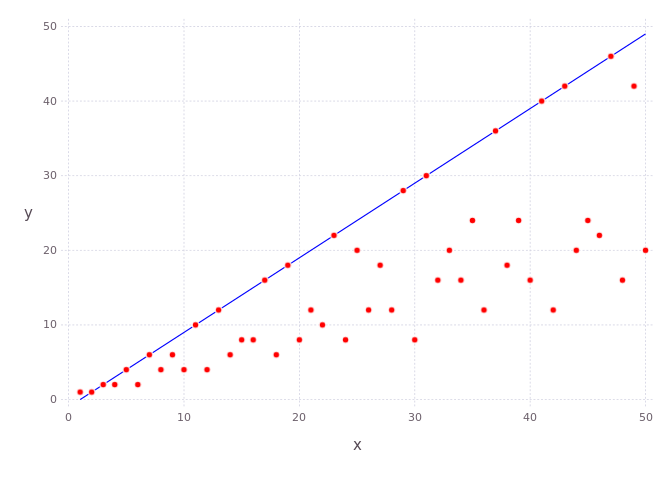
\includegraphics[scale=0.5]{images/euler_phi.png}
\end{figure}


\subsection{Example}

Consider the group $\mZ^\star_{14}$. We have

\begin{verbatim}
Phi(14);
6
\end{verbatim}
%
Therefore the group has $6$ elements (being coprime to 14): $\mZ^\star_{14} = \{1, 3, 5, 9, 11, 13\}$. We can calculate the inverse of a group element using the greatest common divisor as follows

\begin{verbatim}
Gcdex(3,14);
rec( coeff1 := 5, coeff2 := -1, coeff3 := -14, coeff4 := 3, gcd := 1 )
\end{verbatim}
%
So we have $ux + vy = 5 \times 3 + (-1) \times 14 = \gcd(3,14) = 1$. Looking at \eqref{gcd_01:inv}, we see that $u$ is the desired inverse which in this case is $u=5$; i.e. we have $3 \times 5 \equiv 1 \bmod 14$. For the other group elements we obtain

\begin{verbatim}
gap> Gcdex(5,14);
rec( coeff1 := 3, coeff2 := -1, coeff3 := -14, coeff4 := 5, gcd := 1 )
\end{verbatim}
%
so we get $5^{-1} = 3$. The others are a bit more tricky, we have

\begin{verbatim}
gap> Gcdex(9,14);
rec( coeff1 := -3, coeff2 := 2, coeff3 := 14, coeff4 := -9, gcd := 1 )
gap> Gcdex(11,14);
rec( coeff1 := -5, coeff2 := 4, coeff3 := 14, coeff4 := -11, gcd := 1 )
gap> Gcdex(13,14);
rec( coeff1 := -1, coeff2 := 1, coeff3 := 14, coeff4 := -13, gcd := 1 )
\end{verbatim}
%
where we can make $u$ positive by adding $14$ to it: $9^{-1} = -3 + 14 = 11$, $11^{-1} = -5 + 14 = 9$, $13^{-1} = -1 + 14 = 13$ and - of course - $1^{-1} = 1$.
